\subsection{Collision tests}

\begin{figure}[thb]
    \centering
    \begin{subfigure}[t]{.25\textwidth}
        \centering
        \topinset{(a)}{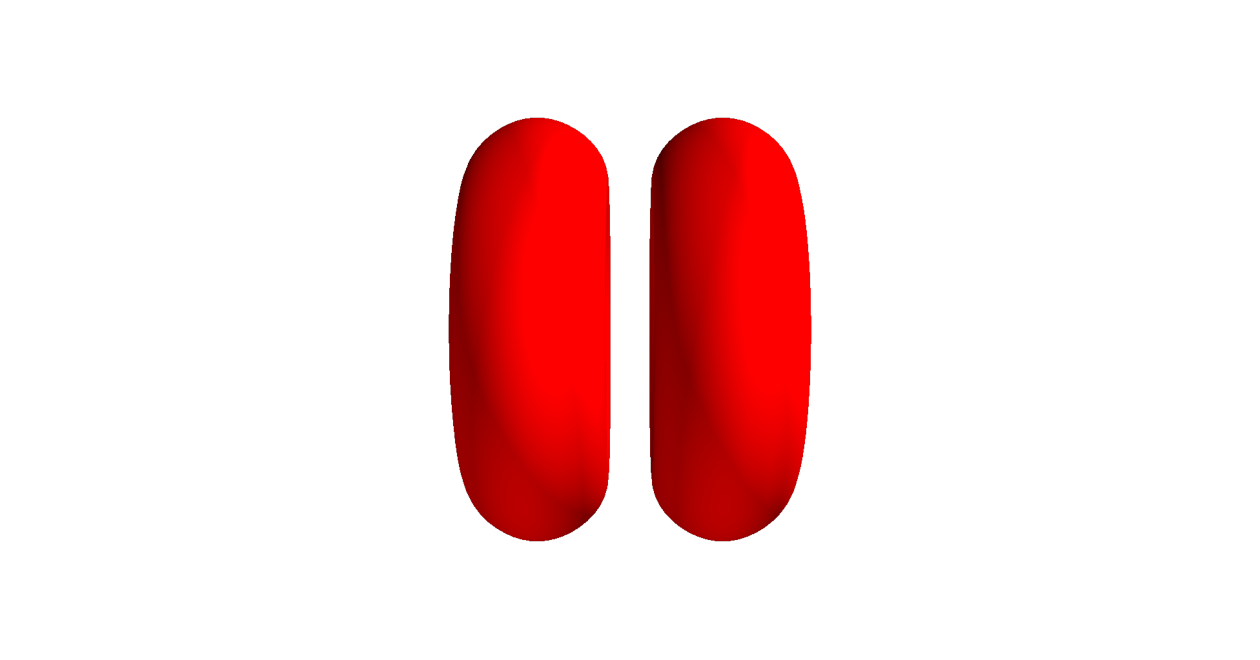
\includegraphics[width=\textwidth]{figures/vvcoll-start.png}}{0.125cm}{0.25cm} \\
        $t = 0\ms$
    \end{subfigure}%
    \begin{subfigure}[t]{.25\textwidth}
        \centering
        \topinset{(b)}{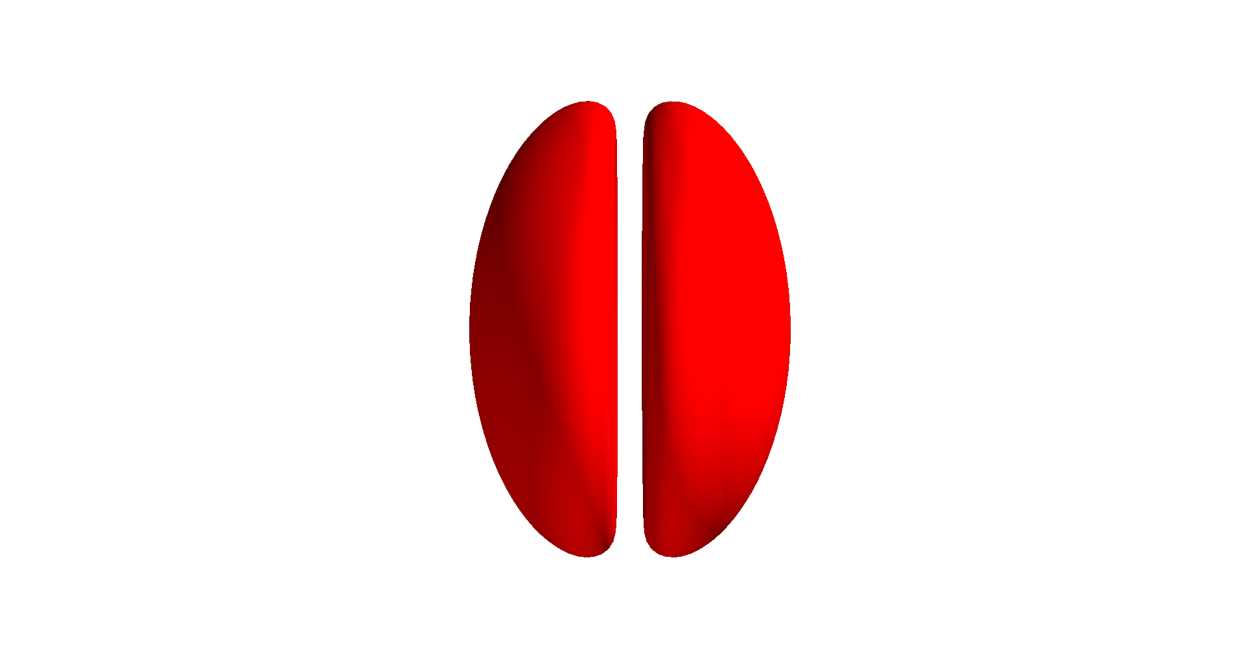
\includegraphics[width=\textwidth]{figures/vvcoll-end.png}}{0.125cm}{0.25cm} \\
        $t = 1.5\ms$
    \end{subfigure}%
    \begin{subfigure}[t]{.25\textwidth}
        \centering
        \topinset{(c)}{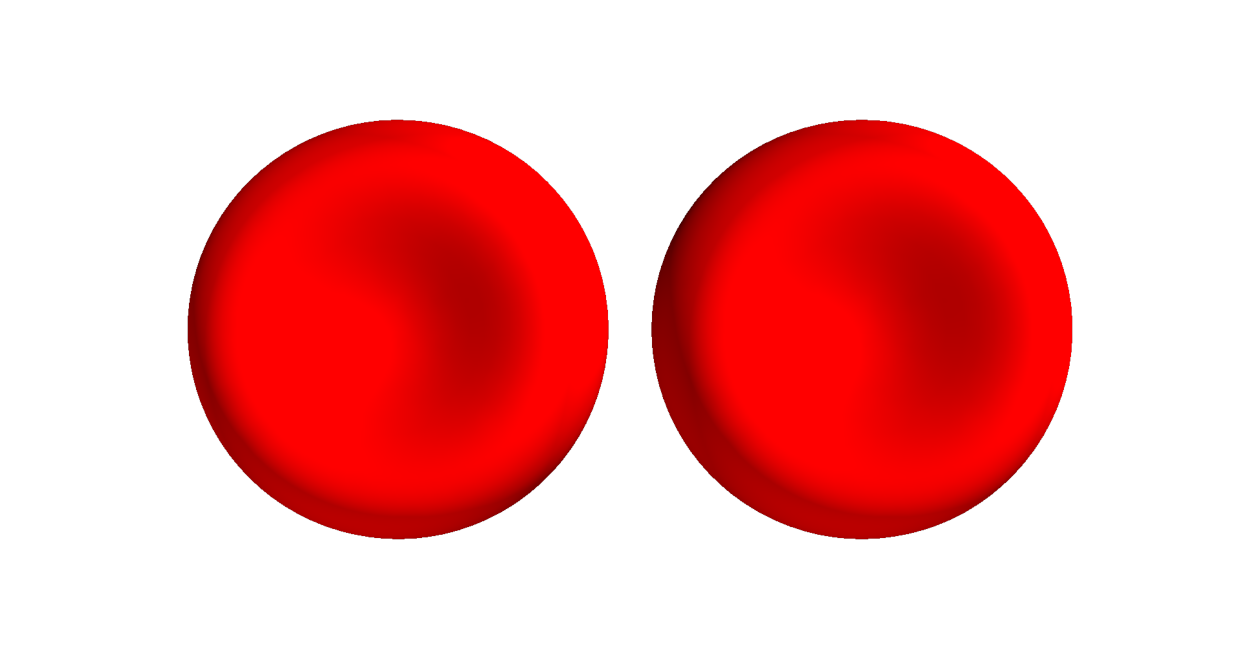
\includegraphics[width=\textwidth]{figures/hhcoll-start.png}}{0.125cm}{0.25cm} \\
        $t = 0\ms$
    \end{subfigure}%
    \begin{subfigure}[t]{.25\textwidth}
        \centering
        \topinset{(d)}{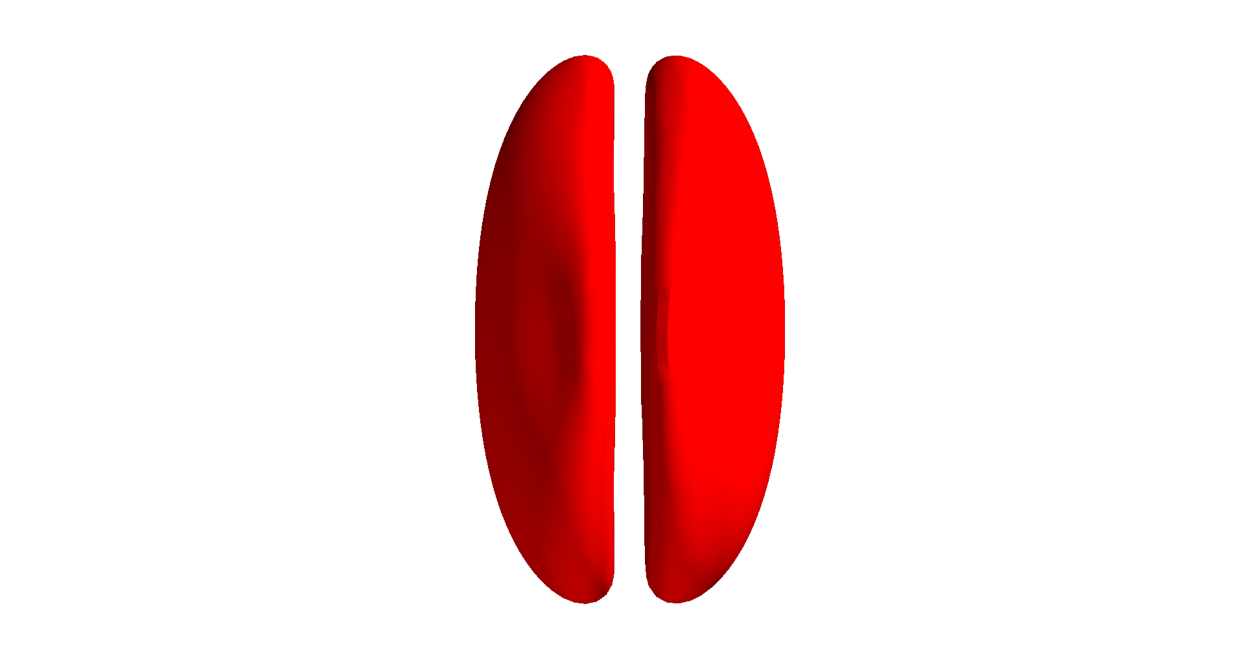
\includegraphics[width=\textwidth]{figures/hhcoll-end.png}}{0.125cm}{0.25cm} \\
        $t = 1.1\ms$
    \end{subfigure}

    \vspace{1em}

    \begin{subfigure}[t]{.25\textwidth}
        \centering
        \topinset{(e)}{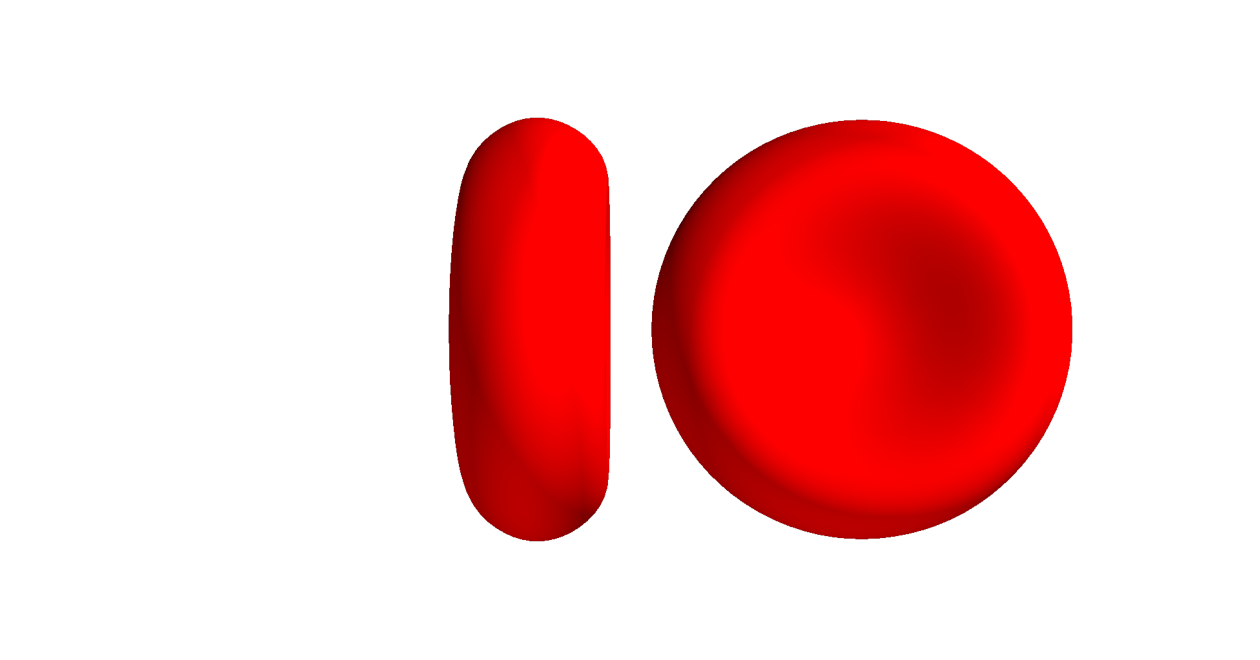
\includegraphics[width=\textwidth]{figures/vhcoll-start.png}}{0.125cm}{0.25cm} \\
        $t = 0\ms$
    \end{subfigure}%
    \begin{subfigure}[t]{.25\textwidth}
        \centering
        \topinset{(f)}{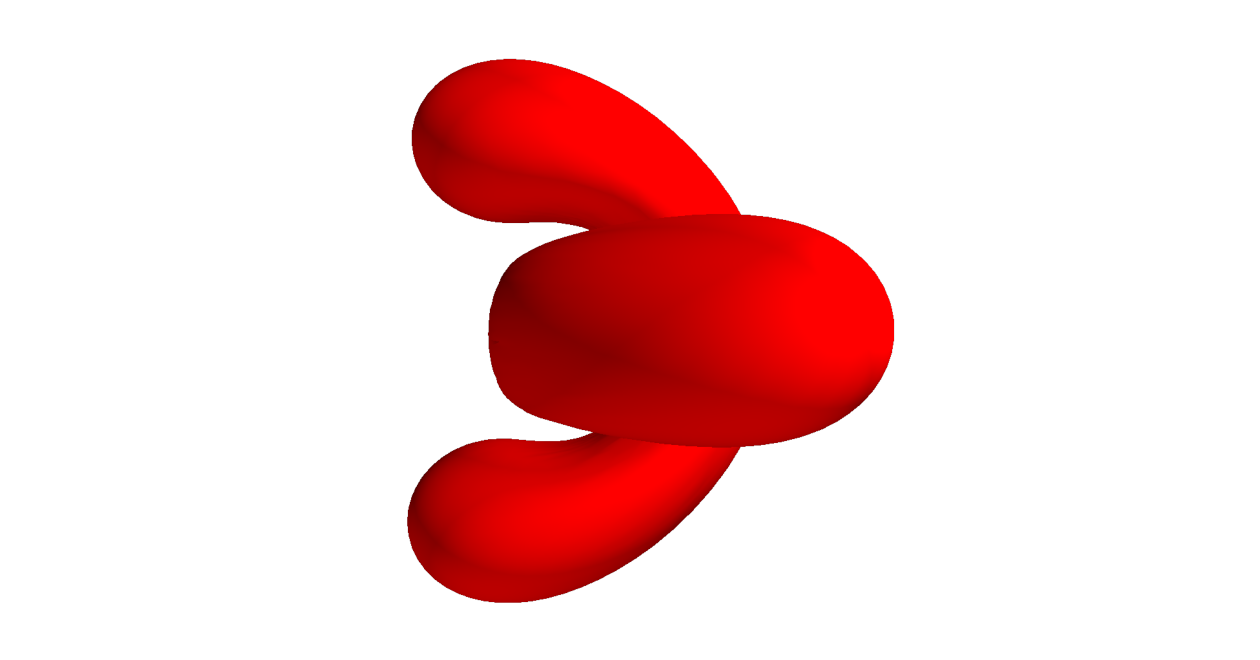
\includegraphics[width=\textwidth]{figures/vhcoll-end.png}}{0.125cm}{0.25cm} \\
        $t = 1.5\ms$
    \end{subfigure}%
    \begin{subfigure}[t]{.25\textwidth}
        \centering
        \topinset{(g)}{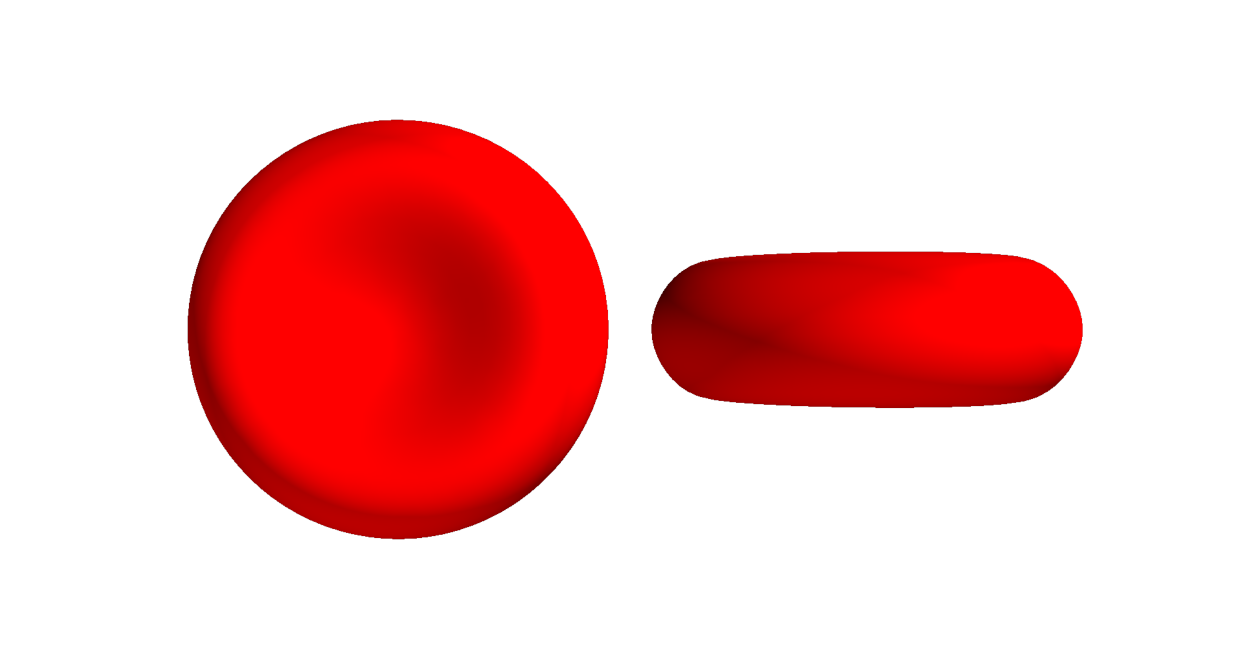
\includegraphics[width=\textwidth]{figures/rhhcoll-start.png}}{0.125cm}{0.25cm} \\
        $t = 0\ms$
    \end{subfigure}%
    \begin{subfigure}[t]{.25\textwidth}
        \centering
        \topinset{(h)}{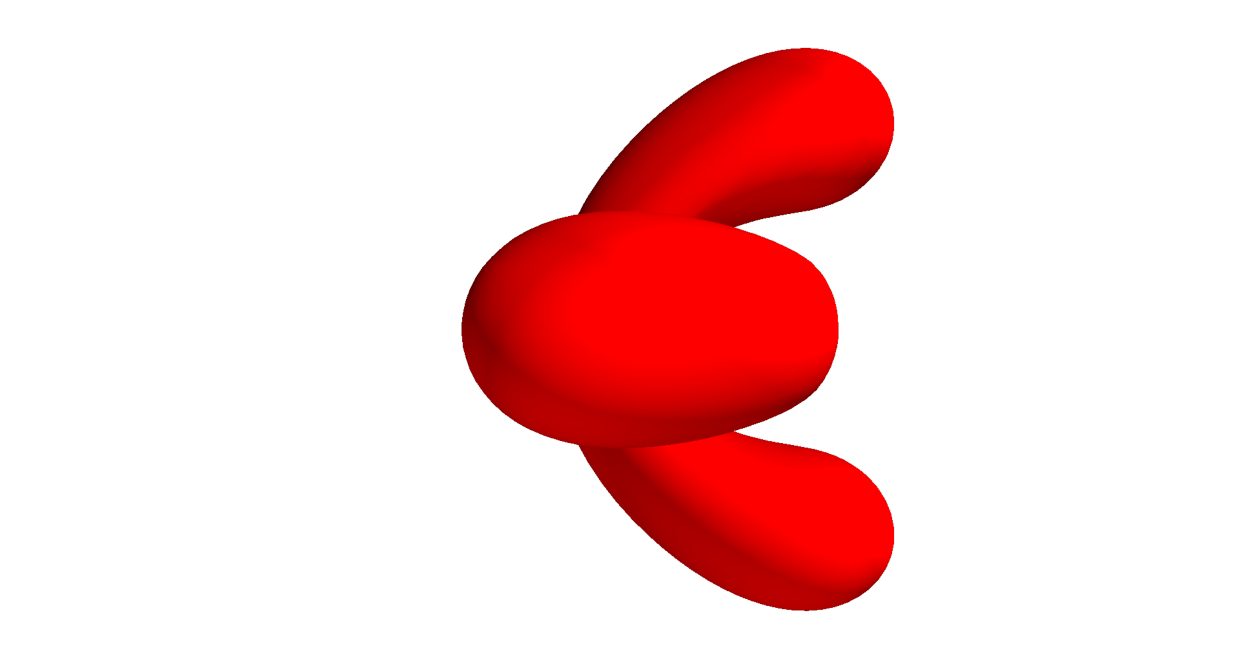
\includegraphics[width=\textwidth]{figures/rhhcoll-end.png}}{0.125cm}{0.25cm} \\
        $t = 1.1\ms$
    \end{subfigure}
    \caption{%
Collision tests between two RBCs. A fictitious force is added to the RBCs to draw them
together. (a--b) The RBCs are initially aligned with concavities facing one another. By
$1.5\ms$, the cells take on a hemispherical shape. The concavities in the gap are
maintained. Shortly thereafter, asymmetries in the setup lead to the cells sliding past
one other. (c--d) The RBCs are initially aligned with their edges facing one
another. By $1.1\ms$, the cells take on a hemispherical shape. The remnants of the
concavity can be seen on the left cell in (d). Shortly thereafter, these cells also slide
past one another. (e--f) The RBCs are initially aligned with the edge of one facing a
concavity of the other. The cells wrap around each other by $1.5\ms$, taking on a bulbous
banana shape. (g--h) The RBCs are initially aligned with their edges facing one another
with one of the cells rotated about the axis $\e_1+\e_3$ by $\pi/2$. By $1.1\ms$, the
cells wrap around each other, again taking on the bulbous banana shape.
    }%
    \label{fig:collisions}
\end{figure}

For the next series of tests, we place two RBCs, with $\data\cardinality=2500$ and
$\sample\cardinality=10000$, in a $16\um\times16\um\times16\um$ domain with periodic
boundaries in the $x^1$ and $x^3$ dimensions and homogeneous Dirichlet boundary
conditions on the $x^2$ dimension. The cells are placed with cell centers on the line
given by $x^1 = x^3$ and $x^2 = 8\um$. The cells are initially separated by a gap of
$4h = 0.8\um$ between their convex hulls, \latin{i.e.}, ignoring the concavities. We add
a fictitious force density
\begin{equation*}
    \F_\text{fict} = \pm 0.1\si{dyn\per\centi\meter}\cdot(\e_1+\e_2)/\sqrt{2},
\end{equation*}
where the sign is chosen so the force points into the gap, to draw the cells together.
Time-stepping uses the 2-stage RK method described in Section~\ref{sec:discretization}.

Initial conditions and configurations after a short time are illustrated in Figure~%
\ref{fig:collisions}. In each case, the cells move slightly closer together and then
undergo considerable deformation. The data sites are initially approximately $2h$ apart
from each other. No problems seem to arise from this. The cells remain distinct, and
the simulations end due to extreme forces triggering our stopping condition.

{\XXX} cosine delta

%max $X^2_\text{rbc} = d = 3.91\um\cdot \sqrt{\tfrac1{35}(55743711 + 7501748\sqrt{974})} / 8750$
